\documentclass[11pt]{article}
\usepackage[margin=1in]{geometry}
\usepackage[utf8]{inputenc}
\usepackage[T1]{fontenc}
\usepackage{enumitem}
\usepackage{hyperref}
\usepackage{xcolor}
\usepackage{titlesec}
\usepackage{tikz}
\usetikzlibrary{positioning, arrows.meta, calc}

\titlespacing*{\section}{0pt}{8pt}{4pt}
\setlength{\parskip}{4pt}
\setlength{\parindent}{0pt}
\pagestyle{empty}

\begin{document}

\begin{center}
{\Large\bfseries Verifier-Backed Defeasible Fine-Tuning}\\[2pt]
{\normalsize Enhancing Foundation Model Performance Where Reward Models Cannot}
\end{center}

\vspace{-3pt}\hrule\vspace{4pt}

\section*{The Problem}

Post-training is the main lever for foundation model capability. Its standard failure modes are well documented: learned reward models drift and get hacked; human preference labelling is slow and noisy; preference and policy optimisation plateau; updates to one capability break unrelated ones. All four trace to one missing ingredient: a fast, exact, model-independent reward signal.

\emph{Defeasible reasoning} provides one. The proof theory admits a polynomial-time verifier that decides, for any candidate hypothesis, whether it resolves an anomaly while preserving every unrelated conclusion (the formal counterpart of AGM minimal change). Plug that verifier in as the reward source for the post-training stack and the four failure modes go away. The verifier never drifts, never approximates, never needs human labelling, and cannot be hacked because it is the proof theory itself.

\section*{The Fine-Tuning Pipeline}

\begin{center}
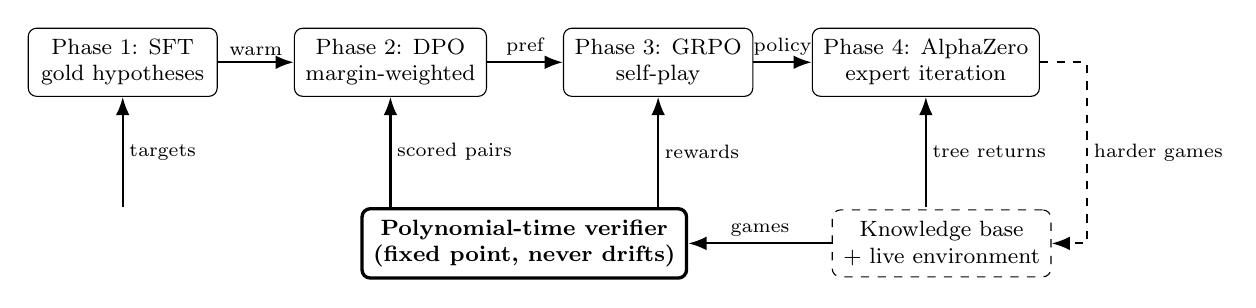
\begin{tikzpicture}[
    >=Latex,
    box/.style={
        draw, rounded corners=3pt,
        minimum height=0.85cm, minimum width=2.4cm,
        font=\footnotesize, inner sep=4pt,
        text centered, align=center
    },
    fixed/.style={
        draw, very thick, rounded corners=3pt,
        minimum height=0.85cm, minimum width=2.6cm,
        font=\footnotesize\bfseries, inner sep=4pt,
        text centered, align=center
    },
    arr/.style={->, thick},
    lbl/.style={font=\scriptsize, inner sep=2pt}
]
    \node[box] (sft) at (0, 0) {Phase 1: SFT\\gold hypotheses};
    \node[box] (dpo) at (3.4, 0) {Phase 2: DPO\\margin-weighted};
    \node[box] (grpo) at (6.8, 0) {Phase 3: GRPO\\self-play};
    \node[box] (az) at (10.2, 0) {Phase 4: AlphaZero\\expert iteration};

    \node[fixed] (ver) at (5.1, -2.3) {Polynomial-time verifier\\(fixed point, never drifts)};
    \node[box, dashed] (kb) at (10.4, -2.3) {Knowledge base\\$+$ live environment};

    \draw[arr] (sft) -- node[lbl, above] {warm} (dpo);
    \draw[arr] (dpo) -- node[lbl, above] {pref} (grpo);
    \draw[arr] (grpo) -- node[lbl, above] {policy} (az);

    \draw[arr] (ver.north -| sft.south) -- (sft.south) node[lbl, midway, right] {targets};
    \draw[arr] (ver.north -| dpo.south) -- (dpo.south) node[lbl, midway, right] {scored pairs};
    \draw[arr] (ver.north -| grpo.south) -- (grpo.south) node[lbl, midway, right] {rewards};
    \draw[arr] (ver.north -| az.south) -- (az.south) node[lbl, midway, right] {tree returns};

    \draw[arr] (kb.west) -- node[lbl, above] {games} (ver.east);
    \draw[arr, dashed] (az.east) -- ++(0.6, 0) |- node[lbl, right, pos=0.25] {harder games} (kb.east);
\end{tikzpicture}
\end{center}

\vspace{-2pt}
{\footnotesize Figure~1. The same verifier scores every stage. Each phase consumes a different shape of verifier output: gold targets for SFT, scored pairs for DPO, group-relative rewards for GRPO, tree-search returns for expert iteration. The model's improvements feed back as harder games. No learned reward model anywhere in the loop.}

\section*{Four Phases, Four Failure Modes Addressed}

\begin{itemize}[nosep, leftmargin=1.4em]
    \item \textbf{SFT on verified gold hypotheses.} Replaces noisy crowd labels with formally verified targets at three difficulty levels. Warm-starts format compliance and grounding.
    \item \textbf{Margin-weighted DPO.} Standard DPO treats every preference pair as equal. The verifier's graded scoring weights each pair by the formal score gap, so the loss puts more gradient on the qualitative transitions (non-resolutive to conservative resolution) than on cosmetic differences. Same DPO objective as everyone else uses; only the labels are formal.
    \item \textbf{GRPO self-play with verifier reward.} Removes the reward-model approximation error of standard RLHF. Self-play produces an automatic curriculum: improvements on one side of a defeasible conflict force improvements on the other. No human curriculum scheduling, no reward hacking.
    \item \textbf{AlphaZero-style expert iteration.} Standard RLVR plateaus once the easy gradient is exhausted (the bottleneck DeepSearch (ICLR 2026) addresses for math). Neural-guided MCTS with the verifier supplying exact terminal scores extends the training surface. Same recipe as AlphaProof's silver-medal IMO result, transposed to a domain where the verifier exists for biomedical, legal, materials, and commonsense reasoning rather than only for formal proofs.
\end{itemize}

\section*{Where Gains Will Show Up}

\begin{itemize}[nosep, leftmargin=1.4em]
    \item \emph{Belief revision under direct prompting.} Current models swing tens of points on exception construction depending on prompting strategy. The capability is latent. Fine-tuning targets the surfacing problem directly.
    \item \emph{Conservativity in updates.} The pathology that breaks ROME, MEMIT and successors is silent disturbance of unrelated conclusions. The verifier scores conservativity directly, so the loss penalises it.
    \item \emph{Headroom on hard subsets.} A pre-registered hard partition stratified along novelty, depth, multi-anomaly, and synthetic contamination is built specifically to expose the gap easy slices hide. It is the surface designed for measuring fine-tuning lift.
    \item \emph{Closed-loop deployment.} A live StarCraft~II bridge runs the same verifier in real-time enforcement. Fine-tuned policies are measurable both on the static benchmark and in closed-loop control under three enforcement modes.
\end{itemize}

\section*{Practical Applications}

The recipe is domain-general; only the knowledge base changes.

\begin{itemize}[nosep, leftmargin=1.4em]
    \item \textbf{Biomedical decision support.} Drug, comorbidity, and pharmacogenomic exception reasoning over UMLS and SNOMED~CT. Confident default-following is the clinically dangerous failure mode.
    \item \textbf{Functional genomics.} Curated negative annotations become first-class fine-tuning signal instead of being silently dropped.
    \item \textbf{Regulatory and legal reasoning.} Conservativity guarantees a fine-tuned compliance agent does not silently invalidate unrelated rulings when one rule changes.
    \item \textbf{Materials and chemistry discovery.} Conjecture refinement with verifier-checked guardrails against false-default predictions.
    \item \textbf{Formal mathematics and program verification.} Same pipeline with Lean's kernel as verifier and Mathlib as the knowledge base.
    \item \textbf{Safety-critical autonomous agents.} Robotics, unmanned systems, and operator-in-the-loop control where every action must be auditable against revisable doctrine.
\end{itemize}

\section*{Why Now}

Verifier-backed RL is the most tractable known route past reward hacking. Defeasible logic is one of the few non-mathematical domains that supplies the polynomial-time exact verifier the recipe requires. The full stack is built, MIT-licensed, and reproducible on commodity HPC.

\end{document}
